\documentclass[]{article}

% Imported Packages
%------------------------------------------------------------------------------
\usepackage{amssymb}
\usepackage{amstext}
\usepackage{amsthm}
\usepackage{amsmath}
\usepackage{enumerate}
%\usepackage{fancyhdr}
\usepackage[margin=1in]{geometry}
\usepackage{graphicx}
%\usepackage{extarrows}
%\usepackage{setspace}
\usepackage{float}
\usepackage[hidelinks]{hyperref}
\usepackage{changebar}

% Configure Packages
%------------------------------------------------------------------------------
\hypersetup{linktoc=all}
\graphicspath{{Resources/}}
%------------------------------------------------------------------------------

% Header and Footer
%------------------------------------------------------------------------------
\pagestyle{plain}



\begin{document}
\cleardoublepage
\pagenumbering{gobble}
\begin{titlepage}
	\newcommand{\HRule}{\rule{\linewidth}{0.5mm}} % Defines a new command
	%for the
	%horizontal lines, change thickness heReve
	\center % Center everything on the page

	%----------------------------------------------------------------------------------------
	%	HEADING SECTIONS
	%----------------------------------------------------------------------------------------

	\textsc{\LARGE McMaster University}\\[1.5cm] % Name of your
	%university/college
	\textsc{\Large Software Design II \\  \Large Large System Design}\\[0.5cm] % Major heading
	%such as course name
	\textsc{\large SFWR ENG 3A04}\\[0.5cm] % Minor heading such as course
	%title

	%----------------------------------------------------------------------------------------
	%	TITLE SECTION
	%----------------------------------------------------------------------------------------

	\HRule \\[0.4cm]
	{ \huge \bfseries SRS Document}\\[0.4cm] % Title of your
	%document
	\HRule \\[1.5cm]

	%----------------------------------------------------------------------------------------
	%	AUTHOR SECTION
	%----------------------------------------------------------------------------------------

	\Large \emph{Authors:}\\
	Alexander \textsc{Jackson} \textbf{1302526} \\
	Harit \textsc{Patel} \textbf{1317372} \\ %Add your student number
	Josh \textsc{Voskamp} \textbf{1319352} \\
	Lucas \textsc{Bongers} \textbf{1202472} \\
	Mohammad \textsc{Naveed} \textbf{1332196} \\[3cm]
	%----------------------------------------------------------------------------------------
	%	DATE SECTION
	%----------------------------------------------------------------------------------------

	{\large \today}\\[3cm] % Date, change the \today to a set date if you
	%want to be precise

	\vfill % Fill the rest of the page with whitespace

\end{titlepage}

% Table of Contents
% Start numbering pages after ToC
\tableofcontents
\cleardoublepage
\pagenumbering{arabic}

\section{Introduction}
\label{sec:introduction}
% Begin Section



\subsection{Purpose}
\label{sub:purpose}
% Begin SubSection

The purpose of this Software Requirements Specification (SRS) document, is to provide the developers with the functional and non-functional requirements that are necessary for the implementation of the system-to-be. Furthermore, the SRS document also provides insight about the constraints that must be adhered to throughout the development life cycle. The intended audience for this SRS document are the developers, TA's, and Dr. Khedri.

% End SubSection
\cbstart
\subsection{Scope}
\label{sub:scope}
% Begin SubSection

The software to be produced is a land-animal identification application for Android devices and will be called, Animaldex. The product will identify a land-animal seen by the user through a series of questions that the software will ask. Depending on the response of the user to these questions, the software will determine what the animal is. The product will only identify the species of the animal, and will not identify the type of the species (i.e. will produce results like Dog and not German Shepherd).
The main objective of the Animaldex application is to be able to provide an accurate answer as to what land-animal the user sees and provide the animal's native region. This application is an asset for people who spend a lot of time outdoors as they can quickly identify animals and further enhance their knowledge about the animals present in their area. Furthermore, younger users can find this application helpful as it can aid their learning and knowledge about land-animals.
\cbend
% End SubSection

\subsection{Definitions, Acronyms, and Abbreviations}
\label{sub:definitions_acronyms_and_abbreviations}
% Begin SubSection
\begin{enumerate}[a)]
%	\item Provide the definitions of all terms, acronyms, and abbreviations required to properly interpret the SRS
	\item\textbf{Welcome Screen:} The screen displayed when the user opens the application. All menu selection is done from here.
	\item\textbf{Experts:} Modules that ask questions about specific aspects of an animal and present a list of possible matches based on the answers provided to it.
	\item\textbf{Animal Identification:} The process started when a user asks the application to help identify an animal.
	\item\textbf{Sighting History:} A list of the last 50 animals sighted by the user.
	\item\textbf{Shape:} One of the experts.
	\item\textbf{Habitat:} One of the experts.
	\item\textbf{Appearance:} One of the experts.
	\item\textbf{Possible Matches:} The list of possible animals the experts have narrowed the search down to based on the answers provided by the user.
	\item\textbf{Central Forum:} The location that all experts send their possible matches to, this screen is diplayed after all the experts have finished formulating their possible matches.
	\item\textbf{Danger Rating:} The potential danger that an identified animal can pose to humans in a worst case scenario.
	\item\textbf{Correct Match:} An entry from the list of possible matches that matches the animal the user described.
	\item\textbf{Incorrect Match:} An entry from the list of possible matches that does not match the animal the user described.
	\item\textbf{User Interface (UI):} The system in which the user interacts and communicates with the application.
	\item\textbf{Help Section:} The section that displays a user manual, FAQ's, bug fixes, and a change log.
\end{enumerate}
% End SubSection

\subsection{References}
\label{sub:references}
% Begin SubSection
\begin{itemize}
%	\item Provide a complete list of all documents referenced elsewhere in the SRS
%	\item Identify each document by title, report number (if applicable), date, and publishing organization
%	\item Specify the sources from which the references can be obtained
	\item N/A
\end{itemize}
% End SubSection

\subsection{Overview}
\label{sub:overview}
% Begin SubSection

%	\item Describe what the rest of the SRS contains
%	\item Explain how the SRS is organized
The rest of the SRS contains information about the general overview of the application and both its functional and non-functional requirements. Section 2 of this document is the overall description of the application and includes sections such as the product perspective, constraints, assumptions and dependencies, and so on. Section 3 of the SRS document provides the functional requirements of the application and section 4 provides the non-functional requirements. The last section in the SRS document is a division of labour section that indicates the contributions of each individual to this document.

% End SubSection

% End Section

\section{Overall Description}
\label{sec:overall_description}
% Begin Section

%This section of the SRS should describe the general factors that affect the product and its requirements. It does not state specific requirements; it provides a background for those requirements and makes them easier to understand.

\cbstart
\subsection{Product Perspective}
\label{sub:product_perspective}
% Begin SubSection
\begin{enumerate}[a)]
%%%%%%%%%%%%%%%%%%%%%%%%%%%%%%%%%%%%%%%%%%%%%%%%%%%%%%%%%%%%%%%%%%%%%%%%%%%%%%%%%%%%%%%%%
%	\item Put the product into perspective with other related products, i.e., context
%	\item If the product is independent and totally self-contained, it should be stated here
%	\item If the SRS defines a product that is a component of a larger system, as frequently occurs, then this subsection should relate the requirements of that larger system to functionality of the software and should identify interfaces between that system and the software
%	\item A block diagram showing the major components of the larger system, interconnections, and external interfaces can be helpful
%%%%%%%%%%%%%%%%%%%%%%%%%%%%%%%%%%%%%%%%%%%%%%%%%%%%%%%%%%%%%%%%%%%%%%%%%%%%%%%%%%%%%%%%%
	\item The application is designed to run on an Android smart-phone. The application will require the use of the Google Maps API, and will depend on the smart-phone having Internet access and location permissions. The application is self contained and does not access any files on the device other than its own.
\end{enumerate}
\cbend
% End SubSection

\subsection{Product Functions}
\label{sub:product_functions}
% Begin SubSection
\begin{enumerate}[a)]
%	\item Provide a summary of the major functions that the software will perform.
%	\begin{itemize}
%		\item \textbf{Example}: An SRS for an accounting program may use this part to address customer account maintenance, customer statement, and invoice preparation without mentioning the vast amount of detail that each of those functions requires.
%	\end{itemize}
%	\item Functions should be organized in a way that makes the list of functions understandable to the customer or to anyone else reading the document for the first time
%	\item Textual or graphical methods can be used to show the different functions and their relationships
%	\begin{itemize}
%		\item Such a diagram is not intended to show a design of a product, but simply shows the logical relationships among variables
%	\end{itemize}
	\item The product shall identify land animals by presenting a series of questions to the user
	\item The product shall determine a list of the closest matches to the answers entered by the user
	\item The product shall display basic information about each of the possible matches
	\item The product shall mark on Google Maps where you were when you sighted the animal
	\item The product shall keep a list of the most recent animals you spotted and their locations
	\item The product shall provide a link to a webpage where the user can find more detailed information about the animal
\end{enumerate}
% End SubSection

\cbstart
\subsection{User Characteristics}
\label{sub:user_characteristics}
% Begin SubSection
\begin{enumerate}[a)]
%%%%%%%%%%%%%%%%%%%%%%%%%%%%%%%%%%%%%%%%%%%%%%%%%%%%%%%%%%%%%%%%%%%%%%%%%%%%%%%%%%%%%%%%
%	\item Describe those general characteristics of the intended users of the product including educational level, experience, and technical expertise
%	\item Do not state specific requirements, but rather provide the reasons why certain specific requirements are later specified
%%%%%%%%%%%%%%%%%%%%%%%%%%%%%%%%%%%%%%%%%%%%%%%%%%%%%%%%%%%%%%%%%%%%%%%%%%%%%%%%%%%%%%%%
	\item The user is expected to comfortable with using and operating an Android smartphone
	\item The user is expected to be proficient in the English langauge
\end{enumerate}
\cbend
% End SubSection

\subsection{Constraints}
\label{sub:constraints}
% Begin SubSection
\begin{enumerate}[a)]
%%%%%%%%%%%%%%%%%%%%%%%%%%%%%%%%%%%%%%%%%%%%%%%%%%%%%%%%%%%%%%%%%%%%%%%%%%%%%%%%%%%%%%%%%
%	\item Provide a general description of any other items that will limit the developer's options
%%%%%%%%%%%%%%%%%%%%%%%%%%%%%%%%%%%%%%%%%%%%%%%%%%%%%%%%%%%%%%%%%%%%%%%%%%%%%%%%%%%%%%%%%
    \item The project must be completed on a budget of \$ 0
    \item Time the project must be finished by April 8th, 2016
\end{enumerate}
% End SubSection

\subsection{Assumptions and Dependencies}
\label{sub:assumptions_and_dependencies}
% Begin SubSection
\begin{enumerate}[a)]
%%%%%%%%%%%%%%%%%%%%%%%%%%%%%%%%%%%%%%%%%%%%%%%%%%%%%%%%%%%%%%%%%%%%%%%%%%%%%%%%%%%%%%%%%
%	\item List each of the factors that affect the requirements stated in the SRS
%	\item These factors are not design constraints on the software but are, rather, any changes to them that can affect the requirements in the SRS
%	\begin{itemize}
%		\item \textbf{Example}: An assumption may be that a specific operating system will be available on the hardware designated for the software product. If, in fact, the operating system is not available, the SRS would then have to change accordingly.
%	\end{itemize}
%%%%%%%%%%%%%%%%%%%%%%%%%%%%%%%%%%%%%%%%%%%%%%%%%%%%%%%%%%%%%%%%%%%%%%%%%%%%%%%%%%%%%%%%%
	\item It is assumed that the device is running Android and has a touch screen
	\item It is assumed that the device is running an Android version of at least 4.1 (Jelly Bean)
	\item It is assumed that the Google Maps API and Services will be available
\end{enumerate}
% End SubSection

\subsection{Apportioning of Requirements}
\label{sub:apportioning_of_requirements}
% Begin SubSection
\begin{enumerate}[a)]
%%%%%%%%%%%%%%%%%%%%%%%%%%%%%%%%%%%%%%%%%%%%%%%%%%%%%%%%%%%%%%%%%%%%%%%%%%%%%%%%%%%%%%%
%	\item Identify requirements that may be delayed until future versions of the system
%%%%%%%%%%%%%%%%%%%%%%%%%%%%%%%%%%%%%%%%%%%%%%%%%%%%%%%%%%%%%%%%%%%%%%%%%%%%%%%%%%%%%%%
    \item The app should be able to identify a wider variety of animals
	\item The app should be able to identify animals from images or videos captured using the device's camera
	\item The app should be able to identify animals from an audio recording
\end{enumerate}
% End SubSection

% End Section
\cbstart
\section{Functional Requirements}
\label{sec:functional_requirements}
% Begin Section
%This section of the SRS should contain all of the software requirements to a level of detail sufficient to enable designers to design a system to satisfy those requirements, and testers to test that the system satisfies those requirements. Throughout this section, every stated requirement should be externally perceivable by users, operators, or other external systems. These requirements should include at a minimum a description of every input (stimulus) into the system, every output (response) from the system, and all functions performed by the system in response to an input or in support of an output.

%You normally have two options for organizing your functional requirements:
%\begin{enumerate}
%	\item Organize first by \emph{business events}, then by \emph{viewpoints}
%	\item Organize first by \emph{viewpoints}, then by \emph{business events}
%\end{enumerate}
%Choose the one which makes the most sense.
%
%For example, if you wish to organization by business events:
\begin{enumerate}[{BE}1.]
	\item User wants to identify an animal
	\begin{enumerate}[{VP1}.1]
		\item User
			\begin{enumerate}
				\item The app must provide a way for the user to open the animal identification service
				\item The app must gather information from the user about the animal
				\item The app must display \textbf{potential matches} based on user input about the animal on the \textbf{central forum}
				\item The active \textbf{experts} must present questions about the different aspects of the animal and its surroundings
				\item The \textbf{experts} must use an algorithm to determine the \textbf{possible matches}
				\item The app must present a way for the user to indicate if the animal is not on the list of \textbf{possible matches}, in which case the identification has failed
				\item The user must be able to select the correct animal from the \textbf{possible matches} if it is there
				\item The app must provide basic information about the selected animal such as habitat, diet, and typical behaviour
				\item The innovative feature must provide information about the \textbf{danger level} of the animal
				\item The app must display buttons for \textbf{Correct Match} and \textbf{Incorrect Match}
			\end{enumerate}
		\item Animal Consultant
			\begin{enumerate}
				\item The animal information algorithm used to identify animals must contain accurate information about the animals with regard to behaviour, diet, and other facts
			\end{enumerate}
		\item Geographic Consultant
			\begin{enumerate}
				\item The animal identification algorithm must be able to be modified in case of changing geographic and climate conditions that affect animal habitat or appearance
			\end{enumerate}
	\end{enumerate}


	\item An attacker wants to breach the system
	\begin{enumerate}[{VP2}.1]
		\item Development Team
			\begin{enumerate}
				\item The messages passed to the \textbf{central forum} by the \textbf{experts} must be encrypted
			\end{enumerate}
		\item Security Consultant
			\begin{enumerate}
					\item The system security designed by the consultant must be able to protect user and app data
			\end{enumerate}
	\end{enumerate}


	\item Development team wants to add/remove experts
	\begin{enumerate}[{VP3}.1]
		\item Development Team
			\begin{enumerate}
				\item The development team must be able to remotely add \textbf{experts} available to the system
				\item The development team must be able to remotely remove \textbf{experts} available to the system
			\end{enumerate}
	\end{enumerate}


	\item User wants to see sighting history
	\begin{enumerate}[{VP4}.1]
		\item User
			\begin{enumerate}
				\item The app must present a way for the user to view the \textbf{sighting history}
				\item The app must show the 50 most recently identified animals
				\item These entries must display the type of animal and date seen, and must be selectable by the user
				\item Upon selection an entry must provide more detailed information about the animal and where it was logged
				\item The entry must include a link directing the user to a site where they can find more detailed information about the animal
				\item the \textbf{sighting history} must provide a way for the user to navigate back to the \textbf{welcome screen}
			\end{enumerate}
	\end{enumerate}


	\item User wants to delete sighting history
	\begin{enumerate}[{VP5}.1]
		\item User
			\begin{enumerate}
				\item The app must provide a way for the user to delete the \textbf{sighting history}
				\item The app must get a yes or no confirmation from the user before deleting the \textbf{sighting history}
				\item If yes is slected the app must delete the \textbf{sighting history}
				\item If no is selcted the app must return the user to the \textbf{welcome screen}
			\end{enumerate}
	\end{enumerate}


	\item User wants to change the experts in use
	\begin{enumerate}[{VP6}.1]
		\item User
			\begin{enumerate}
				\item The app must provide a way for the user to navigate to the \textbf{expert selection} screen
				\item The app must display all \textbf{experts} in the system
				\item The app must display the difference between active and inactive \textbf{experts}
				\item The app must provide a way for the user to activate and deactivate \textbf{experts} to be used
				\item The app must provide a way for the user to return to the \textbf{welcome screen}
			\end{enumerate}
		\end{enumerate}


	\item The user wants to learn more about how to use the app
	\begin{enumerate}[{VP7}.1]
		\item User
			\begin{enumerate}
				\item The app must provide a way for the user to navigate to the \textbf{help section}
				\item The user must be able to view the instruction manual for the app
				\item The user must be able to view frequently asked questions about the app
			\end{enumerate}
		\item Support Team
			\begin{enumerate}
				\item The \textbf{help section} must be updated as new functionalities are added
				\item The \textbf{help section} must display a list of bug fixes and a change log
			\end{enumerate}
	\end{enumerate}
\end{enumerate}
\cbend
% End Section

\section{Non-Functional Requirements}
\label{sec:non-functional_requirements}
% Begin Section
\subsection{Look and Feel Requirements}
\label{sub:look_and_feel_requirements}
% Begin SubSection

\cbstart
\subsubsection{Appearance Requirements}
\label{ssub:appearance_requirements}
% Begin SubSubSection
\begin{enumerate}[{LF}1. ]
	\item The logo and \textbf{user interface} of the application must be visually appealing.
\end{enumerate}
\cbend
% End SubSubSection

\cbstart
\subsubsection{Style Requirements}
\label{ssub:style_requirements}
% Begin SubSubSection
\begin{enumerate}[{LF}2. ]
	\item The \textbf{user interface} of the application must be simple and intuitive.
\end{enumerate}
\cbend
% End SubSubSection

% End SubSection

\subsection{Usability and Humanity Requirements}
\label{sub:usability_and_humanity_requirements}
% Begin SubSection

\cbstart
\subsubsection{Ease of Use Requirements}
\label{ssub:ease_of_use_requirements}
% Begin SubSubSection
\begin{enumerate}[{UH}1. ]
	\item The application must be easy to use without any prior instruction or training.
\end{enumerate}
\cbend
% End SubSubSection

\cbstart
\subsubsection{Personalization and Internationalization Requirements}
\label{ssub:personalization_and_internationalization_requirements}
% Begin SubSubSection
\begin{enumerate}[{UH}2. ]
	\item User profiles must be customizable. The application must support the addition of different languages and multiple in future updates.
\end{enumerate}
\cbend
% End SubSubSection

\subsubsection{Learning Requirements}
\label{ssub:learning_requirements}
% Begin SubSubSection
\begin{enumerate}[{UH}3. ]
	\item No training must be needed to meet the Ease of Use Requirements.
\end{enumerate}
% End SubSubSection

\cbstart
\subsubsection{Understandability and Politeness Requirements}
\label{ssub:understandability_and_politeness_requirements}
% Begin SubSubSection
\begin{enumerate}[{UH}4. ]
	\item The application must be understandable by English-speaking users.
\end{enumerate}
\cbend
% End SubSubSection

\subsubsection{Accessibility Requirements}
\label{ssub:accessibility_requirements}
% Begin SubSubSection
\begin{enumerate}[{UH}5. ]
	\item The application will require an internet connection and permission to use the device's location services.
\end{enumerate}
% End SubSubSection

% End SubSection

\subsection{Performance Requirements}
\label{sub:performance_requirements}
% Begin SubSection

\cbstart
\subsubsection{Speed and Latency Requirements}
\label{ssub:speed_and_latency_requirements}
% Begin SubSubSection
\begin{enumerate}[{PR}1. ]
	\item The application must launch quickly. Queries to \textbf{expert} modules must be returned quickly.
\end{enumerate}
\cbend
% End SubSubSection

\subsubsection{Safety-Critical Requirements}
\label{ssub:safety_critical_requirements}
% Begin SubSubSection
\begin{enumerate}[{PR}2. ]
	\item The application must not cause damage to the device or a loss of data on the device. The applicaiton must not advise or encourage any activity that could bring harm to the user, such as approaching a dangerous animal.
\end{enumerate}
% End SubSubSection

\subsubsection{Precision or Accuracy Requirements}
\label{ssub:precision_or_accuracy_requirements}
% Begin SubSubSection
\begin{enumerate}[{PR}3. ]
	\item The user's detected location must be accurate within 30 metres. Stored information of animals must be consistent with Wikipedia. At least 90\% of final lists of \textbf{possible matches} must include the \textbf{correct match}.
\end{enumerate}
% End SubSubSection

\subsubsection{Reliability and Availability Requirements}
\label{ssub:reliability_and_availability_requirements}
% Begin SubSubSection
\begin{enumerate}[{PR}4. ]
	\item The application must be fully usable 24 hours per day, 7 days per week, as long as the Accessibility Requirements are met.
\end{enumerate}
% End SubSubSection

\subsubsection{Robustness or Fault-Tolerance Requirements}
\label{ssub:robustness_or_fault_tolerance_requirements}
% Begin SubSubSection
\begin{enumerate}[{PR}5. ]
	\item The user must be notified in the event of no \textbf{possible matches}. In the event of an \textbf{incorrect match} or no \text{possible matches}, the user must be allowed to retry.
\end{enumerate}
% End SubSubSection

\subsubsection{Capacity Requirements}
\label{ssub:capacity_requirements}
% Begin SubSubSection
\begin{enumerate}[{PR}6. ]
	\item The \textbf{sighting history} must contain up to 50 animal sightings. The application must contain up to 50 different animals and their information.
\end{enumerate}
% End SubSubSection

\subsubsection{Scalability or Extensibility Requirements}
\label{ssub:scalability_or_extensibility_requirements}
% Begin SubSubSection
\begin{enumerate}[{PR}7. ]
	\item The application's list of known animals must be easily expanded or modified in future updates.
\end{enumerate}
% End SubSubSection

\subsubsection{Longevity Requirements}
\label{ssub:longevity_requirements}
% Begin SubSubSection
\begin{enumerate}[{PR}8. ]
	\item The application must be supported and updated by the development team until at least April 8, 2016.
\end{enumerate}
% End SubSubSection

% End SubSection

\subsection{Operational and Environmental Requirements}
\label{sub:operational_and_environmental_requirements}
% Begin SubSection

\cbstart
\subsubsection{Expected Physical Environment}
\label{ssub:expected_physical_environment}
% Begin SubSubSection
\begin{enumerate}[{OE}1. ]
	\item The application is expected to operate outdoors in all weather conditions.
\end{enumerate}
\cbend
% End SubSubSection

\subsubsection{Requirements for Interfacing with Adjacent Systems}
\label{ssub:requirements_for_interfacing_with_adjacent_systems}
% Begin SubSubSection
\begin{enumerate}[{OE}2. ]
	\item The application must be able to interface with Android and Google Maps without any conflict.
\end{enumerate}
% End SubSubSection

\cbstart
\subsubsection{Productization Requirements}
\label{ssub:productization_requirements}
% Begin SubSubSection
\begin{enumerate}[{OE}3. ]
	\item The application will be released and distributed via Gitlab.
\end{enumerate}
\cbend
% End SubSubSection

\cbstart
\subsubsection{Release Requirements}
\label{ssub:release_requirements}
% Begin SubSubSection
\begin{enumerate}[{OE}4. ]
	\item The application must be fully released on 2016/04/08. This is the final release date.
\end{enumerate}
\cbend
% End SubSubSection

% End SubSection

\subsection{Maintainability and Support Requirements}
\label{sub:maintainability_and_support_requirements}
% Begin SubSection

\cbstart
\subsubsection{Maintenance Requirements}
\label{ssub:maintenance_requirements}
% Begin SubSubSection
\begin{enumerate}[{MS}1. ]
	\item The application must be tested for defects and any found defects must be resolved by 2016/04/08.
\end{enumerate}
\cbend
% End SubSubSection

\cbstart
\subsubsection{Supportability Requirements}
\label{ssub:supportability_requirements}
% Begin SubSubSection
\begin{enumerate}[{MS}2. ]
	\item The application must have an in-application help desk.
\end{enumerate}
\cbend
% End SubSubSection

\cbstart
\subsubsection{Adaptability Requirements}
\label{ssub:adaptability_requirements}
% Begin SubSubSection
\begin{enumerate}[{MS}3. ]
	\item The application must be ported to mobile devices running Android 4.1 Jellybean or later.
\end{enumerate}
\cbend
% End SubSubSection

% End SubSection

\subsection{Security Requirements}
\label{sub:security_requirements}
% Begin SubSection

\subsubsection{Access Requirements}
\label{ssub:access_requirements}
% Begin SubSubSection
\begin{enumerate}[{SR}1. ]
	\item The application must ask the user permission to use the device's location services. A Gitlab account with access to the project repositiory will be required to download the application.
\end{enumerate}
% End SubSubSection

\cbstart
\subsubsection{Integrity Requirements}
\label{ssub:integrity_requirements}
% Begin SubSubSection
\begin{enumerate}[{SR}2. ]
	\item All messages passed to the \textbf{central forum} from the \textbf{expert} modules must be encrypted.
\end{enumerate}
\cbend
% End SubSubSection

\cbstart
\subsubsection{Privacy Requirements}
\label{ssub:privacy_requirements}
% Begin SubSubSection
\begin{enumerate}[{SR}3. ]
	\item The application must not access any files or information that were not created by the application itself.
\end{enumerate}
\cbend
% End SubSubSection

\subsubsection{Audit Requirements}
\label{ssub:audit_requirements}
% Begin SubSubSection
\begin{enumerate}[{SR}1. ]
	\item \emph{N/A}
\end{enumerate}
% End SubSubSection

\subsubsection{Immunity Requirements}
\label{ssub:immunity_requirements}
% Begin SubSubSection
\begin{enumerate}[{SR}2. ]
	\item \emph{N/A}
\end{enumerate}
% End SubSubSection

% End SubSection

\subsection{Cultural and Political Requirements}
\label{sub:cultural_and_political_requirements}
% Begin SubSection

\subsubsection{Cultural Requirements}
\label{ssub:cultural_requirements}
% Begin SubSubSection
\begin{enumerate}[{CP}1. ]
	\item The application must not feature any text, symbols, images, video, or sound that may be deemed offensive by its intended users.
\end{enumerate}
% End SubSubSection

\cbstart
\subsubsection{Political Requirements}
\label{ssub:political_requirements}
% Begin SubSubSection
\begin{enumerate}[{CP}2. ]
	\item \emph{N/A}
\end{enumerate}
\cbend
% End SubSubSection

% End SubSection

\subsection{Legal Requirements}
\label{sub:legal_requirements}
% Begin SubSection

\subsubsection{Compliance Requirements}
\label{ssub:compliance_requirements}
% Begin SubSubSection
\begin{enumerate}[{LR}1. ]
	\item The application must be compliant with all Android, Google Maps, and Gitlab policies.
\end{enumerate}
% End SubSubSection

\subsubsection{Standards Requirements}
\label{ssub:standards_requirements}
% Begin SubSubSection
\begin{enumerate}[{LR}2. ]
	\item The application must display a disclaimer voiding responsibility of the user's interactions with wild animals.
\end{enumerate}
% End SubSubSection

% End SubSection

% End Section


\newpage
\section*{Division of Labour}
\label{sec:division_of_labour}
\addcontentsline{toc}{section}{Division of Labour}
% Begin Section
%Include a Division of Labour sheet which indicates the contributions of each team member. This sheet must be signed by all team members.
\begin{table}[H]
	\centering
	\begin{tabular}{|p{5cm}|p{2cm}|p{3.5cm}|p{3cm}|}\hline
	    Revisions Made & Date & Reason for Revision & Revising Party\\\hline
		Added functional requirements & 2016/01/02 & Document Creation & Lucas Bongers\\\hline
		Added title page, created template & 2016/02/02 & Document Addition & Lucas Bongers\\\hline
		Added non-functional requirements, definition of UI & 2016/02/02 & Document Addition & Alexander Jackson\\\hline
		Added Product Perspective, User Characteristics, Constraints, Assumptions and Dependencies, Apportioning of Requirements, Update template & 2016/02/02 & Document Addition & Josh Voskamp\\\hline
		Added section 1 of SRS document & 2016/02/04 & Document Addition & Mohammad Naveed\\\hline
		Added to Project Perspective & 2016/02/07 & Document Addition & Harit Patel\\\hline
		Corrected some spelling & 2016/02/07 & Spelling & Josh Voskamp\\\hline \cbstart
		Improve Product Perspective, User Characteristics & 2016/02/25 & Correction & Josh Voskamp\\\hline
        Fix Non Functional Req & 2016/02/25 & Correction & Alexander Jackson\\\hline
        Fix Functional Req & 2016/02/25 & Correction & Lucas Bongers\cbend\\\hline
	\end{tabular}
\end{table}

































\section{Introduction}
\label{sec:introduction}
% Begin Section


\subsection{Purpose}
\label{sub:purpose}
% Begin SubSection

The purpose of this document is to provide the developers with the architectural design of the system-to-be. Furthermore, this document also includes diagrams that provide insight on system architecture and structure. The intended audience for this document are the developers, TA's, and Dr. Khedri.

% End SubSection

\subsection{System Description}
\label{sub:system_description}
% Begin SubSection

The application will identify land animals by presenting a series of questions to the user. The application will then produce a list of known animals that best match the answers entered by the user. With each possible match, the application will display basic information about the animal as well as a link to a webpage where the user can find more detailed information. In addition, the application will retain a list of recent animals spotted by the user, including marking on Google Maps the location of the user when each animal was sighted.
\\
\\
The application is designed to run on an Android smart-phone. The application will require the use of the Google Maps API, and will depend on the smart-phone having Internet access and location permissions. The application is designed to be self-contained and will not access any files on the device other than its own.

% End SubSection

\subsection{Overview}
\label{sub:overview}
% Begin SubSection

The rest of this document contains information about the architectural design of the application and its subsytems. Section 2 of this document features a use case diagram of the application, with a text description for each use case, and section 3 contains the corresponding analysis class diagram. Section 4 provides an overview of the overall architectural design of the application. This overview includes justification of the overall architecture, a division of the system into subsystems, and explanation of the relationships between subsystems. Section 6 contains a list of all class responsibility collaboration (CRC) cards, with a CRC card provided for each identified class in the system-to-be. The final section in this document is a division of labour section that indicates the contributions of each individual to this document.

% End SubSection

% End Section

\section{Use Case Diagram}
\label{sec:use_case_diagram}
% Begin Section
%This section should provide a use case diagram for your application.
\begin{figure}[H]
	\centering
	\includegraphics[width = 14cm]{UseCaseDiagram}
	\caption{Use Case Diagram}
	\label{Use Case Diagram}
\end{figure}

\begin{enumerate}[a)]
	\item Help: Lets the user view FAQ's, bug fixes, and change log.

	\item Settings: Section for the user to change app settings: view help menu, view/delete sighting history, select used experts. Extends help section, sighting history, and selecting available experts.

	\item Identify Animal: Starts the animal identification process, includes consult experts and uses location. The results will be displayed to the central forum after the experts have made their decisions.

	\item Consult Experts: A stage in the process of identifying an animal, relies on animal and geographic consultants to ensure accuracy. The experts present a series of questions to the user and decide on possible matches based on the answers.

	\item Sighting History: Contains the most recent animals sighted by the user, and basic information about the animal, and when and where it was sighted. User can delete specific entries or the whole list.

	\item Select Available Experts: Lets the user select which experts to activate/deactivate for use in identifying animals. The user must have at least one expert selected, and cannot choose more than 5 to be in use at a time.

	\item Add Experts: When the development team adds a new expert for users to select for animal identification. The user will be able to select the new expert in the select available experts section.

	\item Remove Experts: When the development team removes an existing expert from the system. The removed expert will no longer be available for selection in the select available experts section, and users who currently have it selected for use will be prompted to select a different expert.

	\item location: The app gets the user's location at the beginning of each animal identification process, and logs it with the animal sighting history.

	\item Encrypt Data: The security consultant must ensure user data and information communicated by the experts is secure
\end{enumerate}
% End Section

\section{Analysis Class Diagram}
\label{sec:analysis_class_diagram}
% Begin Section
% This section should provide an analysis class diagram for your application.
\begin{figure}[H]
	\centering
	\includegraphics[width = 14cm]{ACDV2}
	\caption{Analysis Class Diagram}
	\label{Analysis Class Diagram}
\end{figure}
% End Section


\section{Architectural Design}
\label{sec:architectural_design}
% Begin Section
% This section should provide an overview of the overall architectural design of your application. You overall architecture should show the division of the system into subsystems with high cohesion and low coupling.

\subsection{System Architecture}
\label{sub:system_architecture}
% Begin SubSection
\begin{enumerate}[a)]
	\item The system will be designed using the blackboard version of a data centered architecture.
	\item The agents or knowledge stores of the data store are the experts of the system which will be working independently of each other, they will only interact with the blackboard. When the animal identification process is started the data store will call on the experts to start a decision making process based on the answers the user provides to the questions asked by the experts. The experts will post their decisions to the central forum for the user to view after the process has been completed. The blackboard will contain the knowledge entered by the user, and the experts will contain the rules used to sort the knowledge contained in the blackboard.
	\item The system will use the blackboard style architecture because the app is based on a decision making process. The experts may not always agree on the result since they are all contributing and drawing from different areas of knowledge, and so they will all contribute different views. The most likely of these views are the ones that will be posted to the central forum for the user to view.
\end{enumerate}
\begin{figure}[H]
	\centering
	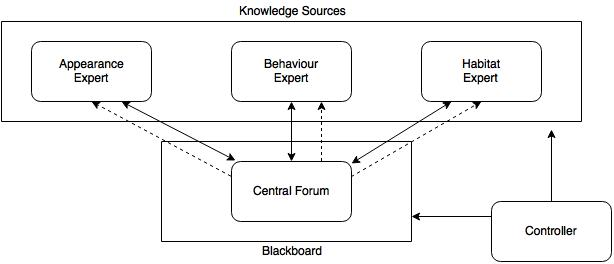
\includegraphics[width = 14cm]{Subsystem_Architecture}
	\caption{Subsystem Architecture}
	\label{Subsystem Architecture}
\end{figure}
% End SubSection

\subsection{Subsystems}
\label{sub:subsystems}
% Begin SubSection
\begin{enumerate}[a)]
	\item Blackboard Subsystem: The purpose of this system is to store all the knowledge and to call on the experts to reach decisions based on the knowledge in the central forum. It prompts the knowledge source subsystem and is controlled by the controller subsystem.
	\item Knowledge Subsystem: The purpose of this system is to make decisions on the data contained in the data store when prompted by the blackboard. The classes in the knowledge source subsystem communicate only with the blackboard and not with each other. This subsystem is prompted by the blackboard subsystem and controlled by the controller subsystem.
	\item Controller Subsystem: The responsibility of this system is to have overall supervision of the entire system and to initiate the knowledge and blackboard subsystems.
\end{enumerate}
% End SubSection

% End Section

\section{Class Responsibility Collaboration (CRC) Cards}
\label{sec:class_responsibility_collaboration_crc_cards}
% Begin Section
%This section should contain all of your CRC cards.

% \begin{enumerate}[a)]
% 	\item Provide a CRC Card for each identified class
% 	\item Please use the format outlined in tutorial, i.e.,
% 	\begin{table}[ht]
% 		\centering
% 		\begin{tabular}{|p{5cm}|p{5cm}|}
% 		\hline
% 		 \multicolumn{2}{|l|}{\textbf{Class Name:}} \\
% 		\hline
% 		\textbf{Responsibility:} & \textbf{Collaborators:} \\
% 		\hline
% 		\vspace{1in} & \\
% 		\hline
% 		\end{tabular}
% 	\end{table}
%
% \end{enumerate}
\begin{table}[H]
	\centering
	\begin{tabular}{|p{5cm}|p{5cm}|}
		\hline
		\multicolumn{2}{|l|}{\textbf{IdentificationControl}} \\
		\hline
		\textbf{Responsibility:} & \textbf{Collaborators:} \\
		\hline
		 Controller class that calls collaborators to identify an animal and passes results to GUIControl to display results and store result in sighting history & BehaviourExpertControl \break AppearanceExpertControl \break HabitatExpertControl \break GUIControl\\
		\hline
	\end{tabular}
\end{table}
\begin{table}[H]
	\centering
	\begin{tabular}{|p{5cm}|p{5cm}|}
		\hline
		\multicolumn{2}{|l|}{\textbf{BehaviourExpertControl}} \\
		\hline
		\textbf{Responsibility:} & \textbf{Collaborators:} \\
		\hline
		 Controller class that controls interactions and requests for the Behaviour Expert & BehaviourExpertEntity \break IdentificationControl\\
		\hline
	\end{tabular}
\end{table}
\begin{table}[H]
	\centering
	\begin{tabular}{|p{5cm}|p{5cm}|}
		\hline
		\multicolumn{2}{|l|}{\textbf{AppearanceExpertControl}} \\
		\hline
		\textbf{Responsibility:} & \textbf{Collaborators:} \\
		\hline
		 Controller class that controls interactions and requests for the Appearance Expert & AppearanceExpertEntity \break IdentificationControl\\
\hline
	\end{tabular}
\end{table}
\begin{table}[H]
	\centering
	\begin{tabular}{|p{5cm}|p{5cm}|}
		\hline
		\multicolumn{2}{|l|}{\textbf{HabitatExpertControl}} \\
		\hline
		\textbf{Responsibility:} & \textbf{Collaborators:} \\
		\hline
		 Controller class that controls interactions and requests for the Habitat Expert & HabitatExpertEntity \break IdentificationControl\\
\hline
	\end{tabular}
\end{table}
\begin{table}[H]
	\centering
	\begin{tabular}{|p{5cm}|p{5cm}|}
		\hline

		\multicolumn{2}{|l|}{\textbf{BehaviourExpertEntity}} \\
		\hline
		\multicolumn{2}{|l|}{\textbf{SightingHistroy}} \\\hline
		\textbf{Responsibility:} & \textbf{Collaborators:} \\
		\hline
		 Entity class that contains information necessary to identify animal based on its behaviour & BehaviourExpertControl\\
\hline
	\end{tabular}
\end{table}
\begin{table}[H]
	\centering
	\begin{tabular}{|p{5cm}|p{5cm}|}
		\hline
		\multicolumn{2}{|l|}{\textbf{AppearanceExpertEntity}} \\
		\hline
		\textbf{Responsibility:} & \textbf{Collaborators:} \\
		\hline
		 Entity class that contains information necessary to identify animal based on its appearance & AppearanceExpertControl\\
		\hline

	\end{tabular}
\end{table}
\begin{table}[H]
	\centering
	\begin{tabular}{|p{5cm}|p{5cm}|}
		\hline
		\multicolumn{2}{|l|}{\textbf{HabitatExpertEntity}} \\
		\hline
		\textbf{Responsibility:} & \textbf{Collaborators:} \\
		\hline
		 Entity class that contains information necessary to identify animal based on its habitat & HabitatExpertControl\\
\hline
	\end{tabular}
\end{table}
\begin{table}[H]
	\centering
	\begin{tabular}{|p{5cm}|p{5cm}|}
		\hline
		\multicolumn{2}{|l|}{\textbf{GUIControl}} \\
		\hline
		\textbf{Responsibility:} & \textbf{Collaborators:} \\
		\hline
		 Controller class that interfaces  between the animal identification process and the UI classes and home screen & IdentificationControl \break Results \break SightingHistory \break SelectExperts \break AnswerQuestion \break Help \break IdentifyAnimal \break Settings\\
\hline
	\end{tabular}
\end{table}
\begin{table}[H]
	\centering
	\begin{tabular}{|p{5cm}|p{5cm}|}
		\hline
		\multicolumn{2}{|l|}{\textbf{Results}} \\
		\hline
		\textbf{Responsibility:} & \textbf{Collaborators:} \\
		\hline
		Show results of animal identification process and allow user to select correctly identified animal from list & GUIControl\\
		\hline

	\end{tabular}
\end{table}
\begin{table}[H]
	\centering
	\begin{tabular}{|p{5cm}|p{5cm}|}
		\hline
		\multicolumn{2}{|l|}{\textbf{SightingHistory}} \\
		\hline
		\textbf{Responsibility:} & \textbf{Collaborators:} \\
		\hline
		 Allows user to view and delete animal sighting history & GUIControl \\
\hline
	\end{tabular}
\end{table}
\begin{table}[H]
	\centering
	\begin{tabular}{|p{5cm}|p{5cm}|}
		\hline
		\multicolumn{2}{|l|}{\textbf{SelectExperts}} \\
		\hline
		\textbf{Responsibility:} & \textbf{Collaborators:} \\
		\hline
		 Lets user select which experts will be called on during future animal identification processes & GUIControl \\
\hline
	\end{tabular}
\end{table}
\begin{table}[H]
	\centering
	\begin{tabular}{|p{5cm}|p{5cm}|}
		\hline
		\multicolumn{2}{|l|}{\textbf{AnswerQuestion}} \\
		\hline
		\textbf{Responsibility:} & \textbf{Collaborators:} \\
		\hline
		 Allows user to answer question presented by experts during the animal identification process & GUIControl \\
\hline
	\end{tabular}
\end{table}
\begin{table}[H]
	\centering
	\begin{tabular}{|p{5cm}|p{5cm}|}
		\hline
		\multicolumn{2}{|l|}{\textbf{Help}} \\
		\hline
		\textbf{Responsibility:} & \textbf{Collaborators:} \\
		\hline
		 Boundary class that displays help information such as FAQs, how to use the app and troubleshooting & GUIControl\\
		\hline
	\end{tabular}
\end{table}
\begin{table}[H]
	\centering
	\begin{tabular}{|p{5cm}|p{5cm}|}
		\hline
		\multicolumn{2}{|l|}{\textbf{IdentifyAnimal}} \\
		\hline
		\textbf{Responsibility:} & \textbf{Collaborators:} \\
		\hline
		 Allows user to begin the animal identification process & GUIControl \\
\hline
	\end{tabular}
\end{table}

% End Section

\newpage
\section*{Division of Labour}
\label{sec:division_of_labour}
\addcontentsline{toc}{section}{Division of Labour}
% Begin Section
%Include a Division of Labour sheet which indicates the contributions of each team member. This sheet must be signed by all team members.
\begin{table}[H]
	\centering
	\begin{tabular}{|p{5cm}|p{2cm}|p{3.5cm}|p{3cm}|}\hline
	    \textbf{Revisions Made} & \textbf{Date} & \textbf{Reason for Revision} & \textbf{Revising Party}\\\hline
		Added title page & 2016/02/11 & Document Creation & Josh Voskamp\\\hline
		Added introduction & 2016/03/03 & Document Addition & Alexander Jackson\\\hline
		Added use case descriptions, system architecture and diagram, and subsystem breakdown & 2016/03/05 & Document Addition & Lucas Bongers\\\hline
		Added Use Case Diagram, Analysis Class Diagram, CRC Cards & 2016/03/05 & Document Addition & Josh Voskamp, \break Mohammad Naveed, \break Harit Patel\\\hline
		Added new version of analysis class diagram & 2016/03/17 & Document Addition & Lucas Bongers\\\hline
		Changed all CRC cards based on new analysis class diagram & 2016/03/17 & Document Addition & Lucas Bongers\\\hline
	\end{tabular}
\end{table}





































\section{Introduction}
\label{sec:introduction}
% Begin Section


\subsection{Purpose}
\label{sub:purpose}
% Begin SubSection

The purpose of this document is to provide the developers with a more detailed design of the system-to-be. Furthermore, this document also includes diagrams that provide insight on system states and classes. The intended audience for this document are the developers, TA's, and Dr. Khedri.

% End SubSection

\subsection{System Description}
\label{sub:system_description}
% Begin SubSection

The application will identify land animals by presenting a series of questions to the user. The application will then produce a list of known animals that best match the answers entered by the user. With each possible match, the application will display basic information about the animal as well as a link to a webpage where the user can find more detailed information. In addition, the application will retain a list of recent animals spotted by the user, including marking on Google Maps the location of the user when each animal was sighted.
\\
\\
The application is designed to run on an Android smart-phone. The application will require the use of the Google Maps API, and will depend on the smart-phone having Internet access and location permissions. The application is designed to be self-contained and will not access any files on the device other than its own.

% End SubSection

\subsection{Overview}
\label{sub:overview}
% Begin SubSection

The rest of this document contains information about the detailed design of the application and its classes. Section 2 of this document features a state chart for each controller class of the application, and section 3 contains a sequence diagram for each use case of the application. Section 4 provides a detailed class diagram for the application. The final section of this document is a division of labour table that indicates the contributions of each individual to this document.

% End SubSection

% End Section

\section{State Charts for Controller Classes}
\label{sec:state_charts_for_controller_classes}
% Begin Section
\begin{figure}[H]
	\addcontentsline{toc}{figure}{GUI controller}
	\centering
	\includegraphics[width = 14cm]{GUIControlStateChart}
	\caption{State Chart Diagram for GUI controller}
	\label{State Chart Diagram for GUI controller}
\end{figure}

\begin{figure}[H]
	\addcontentsline{toc}{figure}{Animal Identification Controller}
	\centering
	\includegraphics[width = 7cm]{IdentificationStateChart}
	\caption{State Chart Diagram for Animal Identification Controller}
	\label{State Chart Diagram for Animal Identification Controller}
\end{figure}

\begin{figure}[H]
	\addcontentsline{toc}{figure}{Each Expert Controller}
	\centering
	\includegraphics[width = 7cm]{ExpertStateChart}
	\caption{State Chart Diagram for each Expert, i Controller}
	\label{State Chart Diagram for each Expert, i Controller}
\end{figure}

% End Section

\section{Sequence Diagrams}
\label{sec:sequence_diagrams}
% Begin Section
%This section should provide a use case diagram for your application.
\begin{figure}[H]
	\addcontentsline{toc}{figure}{Identify Animal}
	\centering
	\includegraphics[width = 14cm]{IDAnimalSequenceDiagram}
	\caption{Identify Animal Sequence Diagram}
	\label{Identify Animal Sequence Diagram}
\end{figure}

\begin{figure}[H]
	\addcontentsline{toc}{figure}{Select Experts}
	\centering
	\includegraphics[width = 7cm]{SelectExpertsSequenceDiagram}
	\caption{Select Experts Sequence Diagram}
	\label{Select Experts Sequence Diagram}
\end{figure}

\begin{figure}[H]
	\addcontentsline{toc}{figure}{View Help}
	\centering
	\includegraphics[width = 4.5cm]{ViewHelpSequenceDiagram}
	\caption{View Help Sequence Diagram}
	\label{View Help Sequence Diagram}
\end{figure}

\begin{figure}[H]
	\addcontentsline{toc}{figure}{View Sighting History}
	\centering
	\includegraphics[width = 5cm]{ViewSightingHistorySequenceDiagram}
	\caption{View Sighting History Sequence Diagram}
	\label{View Sighting History Sequence Diagram}
\end{figure}

\begin{figure}[H]
	\addcontentsline{toc}{figure}{Delete Sighting History}
	\centering
	\includegraphics[width = 7cm]{DeleteSightingHistorySequenceDiagram}
	\caption{Delete Sighting History Sequence Diagram}
	\label{Delete Sighting History Sequence Diagram}
\end{figure}

% End Section

\section{Detailed Class Diagram}
\label{sec:detailed_class_diagram}
\begin{figure}[H]
	\centering
	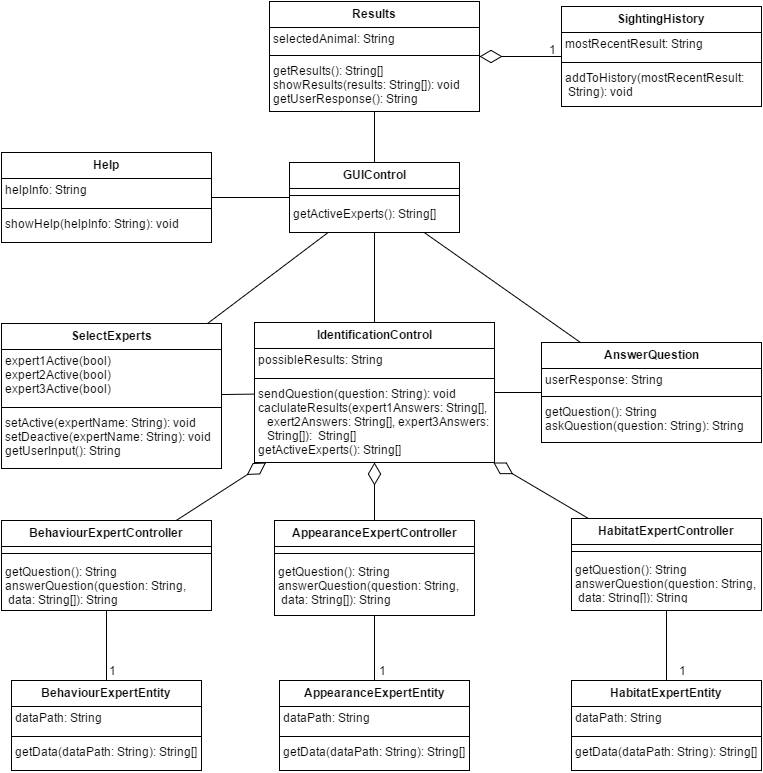
\includegraphics[width = 14cm]{DetailedClassDiagram}
	\caption{Detailed Class Diagram}
	\label{Detailed Class Diagram}
\end{figure}
% Begin Section
%This section should provide a use case diagram for your application.

% End Section


\newpage
\section*{Division of Labour}
\label{sec:division_of_labour}
\addcontentsline{toc}{section}{Division of Labour}
% Begin Section
%Include a Division of Labour sheet which indicates the contributions of each team member. This sheet must be signed by all team members.
\begin{table}[H]
	\centering
	\begin{tabular}{|p{5cm}|p{2cm}|p{3.5cm}|p{3cm}|}\hline
	    \textbf{Revisions Made} & \textbf{Date} & \textbf{Reason for Revision} & \textbf{Revising Party}\\\hline
		Added title page and introduction & 2016/03/22 & Document Creation & Alexander Jackson\\\hline
		Sequence Diagrams & 2016/03/22 & Document Addition & Josh Voskamp, Harit Patel, Mohammad Naveed\\\hline
		Added state chart diagrams & 2016/03/24 & Document Addition & Lucas Bongers\\\hline
		Created Detailed Class Diagram & 2016/03/27 & Document Addition & Harit Patel, Lucas Bongers, Alexander Jackson\\\hline
		Spelling Fixes & 2016/03/27 & Corrections & Josh Voskamp\\\hline
	\end{tabular}
\end{table}


\end{document}
%------------------------------------------------------------------------------


